\begin{frame}
\frametitle{Exploring The Data: Terrorist Relations I}
	
	\begin{itemize}
		\item  Each node is a relation between two terrorists
		\item  Nodes are connected if they share one individual
		\item  Relation type and binary vector of features for each node
		\item  Line graph
	\end{itemize}
	
	\begin{figure}
		\begin{center}
			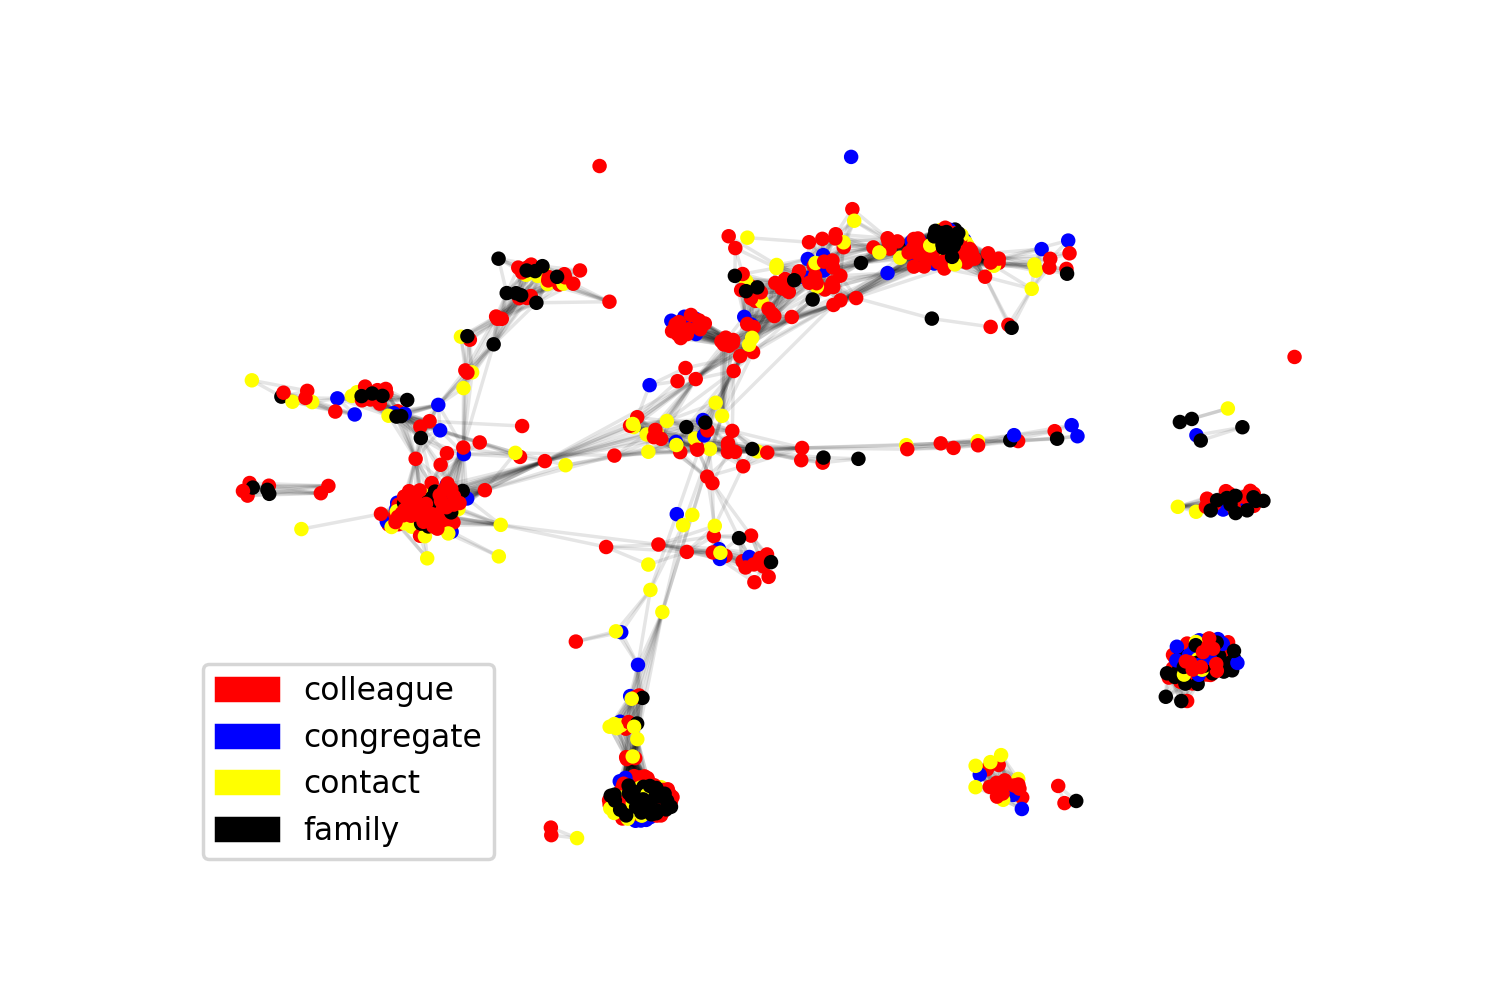
\includegraphics[width=.5\textwidth]{graphRel.png}
			\caption{Graph of the terrorist relations dataset}
			\label{fig:graph relations}
		\end{center}
	\end{figure}
	
\end{frame}

\begin{frame}
\frametitle{Exploring The Data: What Is a Line Graph?}

\begin{definition}
	Given a graph $\mathcal{G}$, its line graph $L\{\mathcal{G}\}$ is defined as follows: 
	\begin{itemize}
		\item Each node of $L\{\mathcal{G}\}$ stands for an edge of $\mathcal{G}$
		\item Two nodes of $L\{\mathcal{G}\}$ are connected $\Leftrightarrow$ they share a node of $\mathcal{G}$
	\end{itemize}
\end{definition}

\begin{figure}
		\begin{center}
			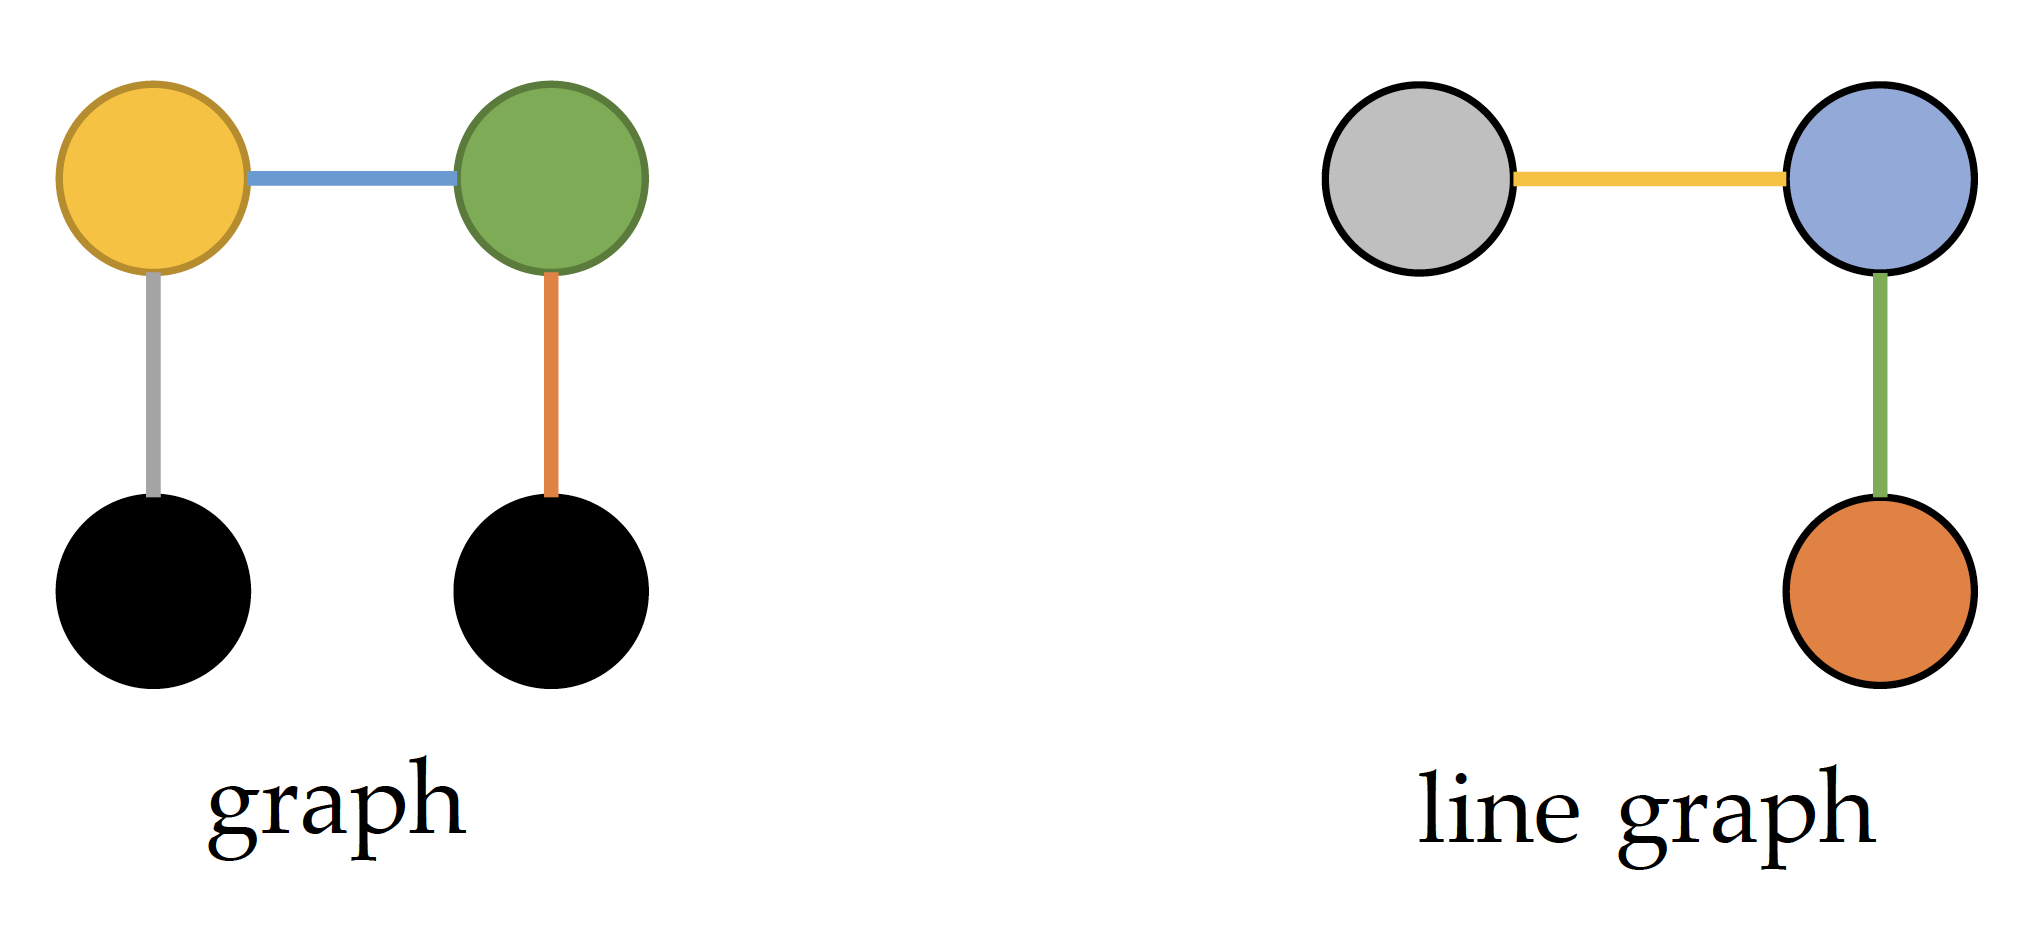
\includegraphics[width=.5\textwidth]{linegraph}
			\caption{Construction of a line graph}
			\label{fig:line graph}
		\end{center}
	\end{figure}

\end{frame}

\begin{frame}
\frametitle{Exploring The Data: Terrorist Attacks I}
	
	\begin{itemize}
		\item Each node is an attack
		\item Nodes are connected if the attacks were in close locations
		\item Location, date, organisation and binary vector of features for each node
	\end{itemize}
	
	\begin{figure}
		\begin{center}
			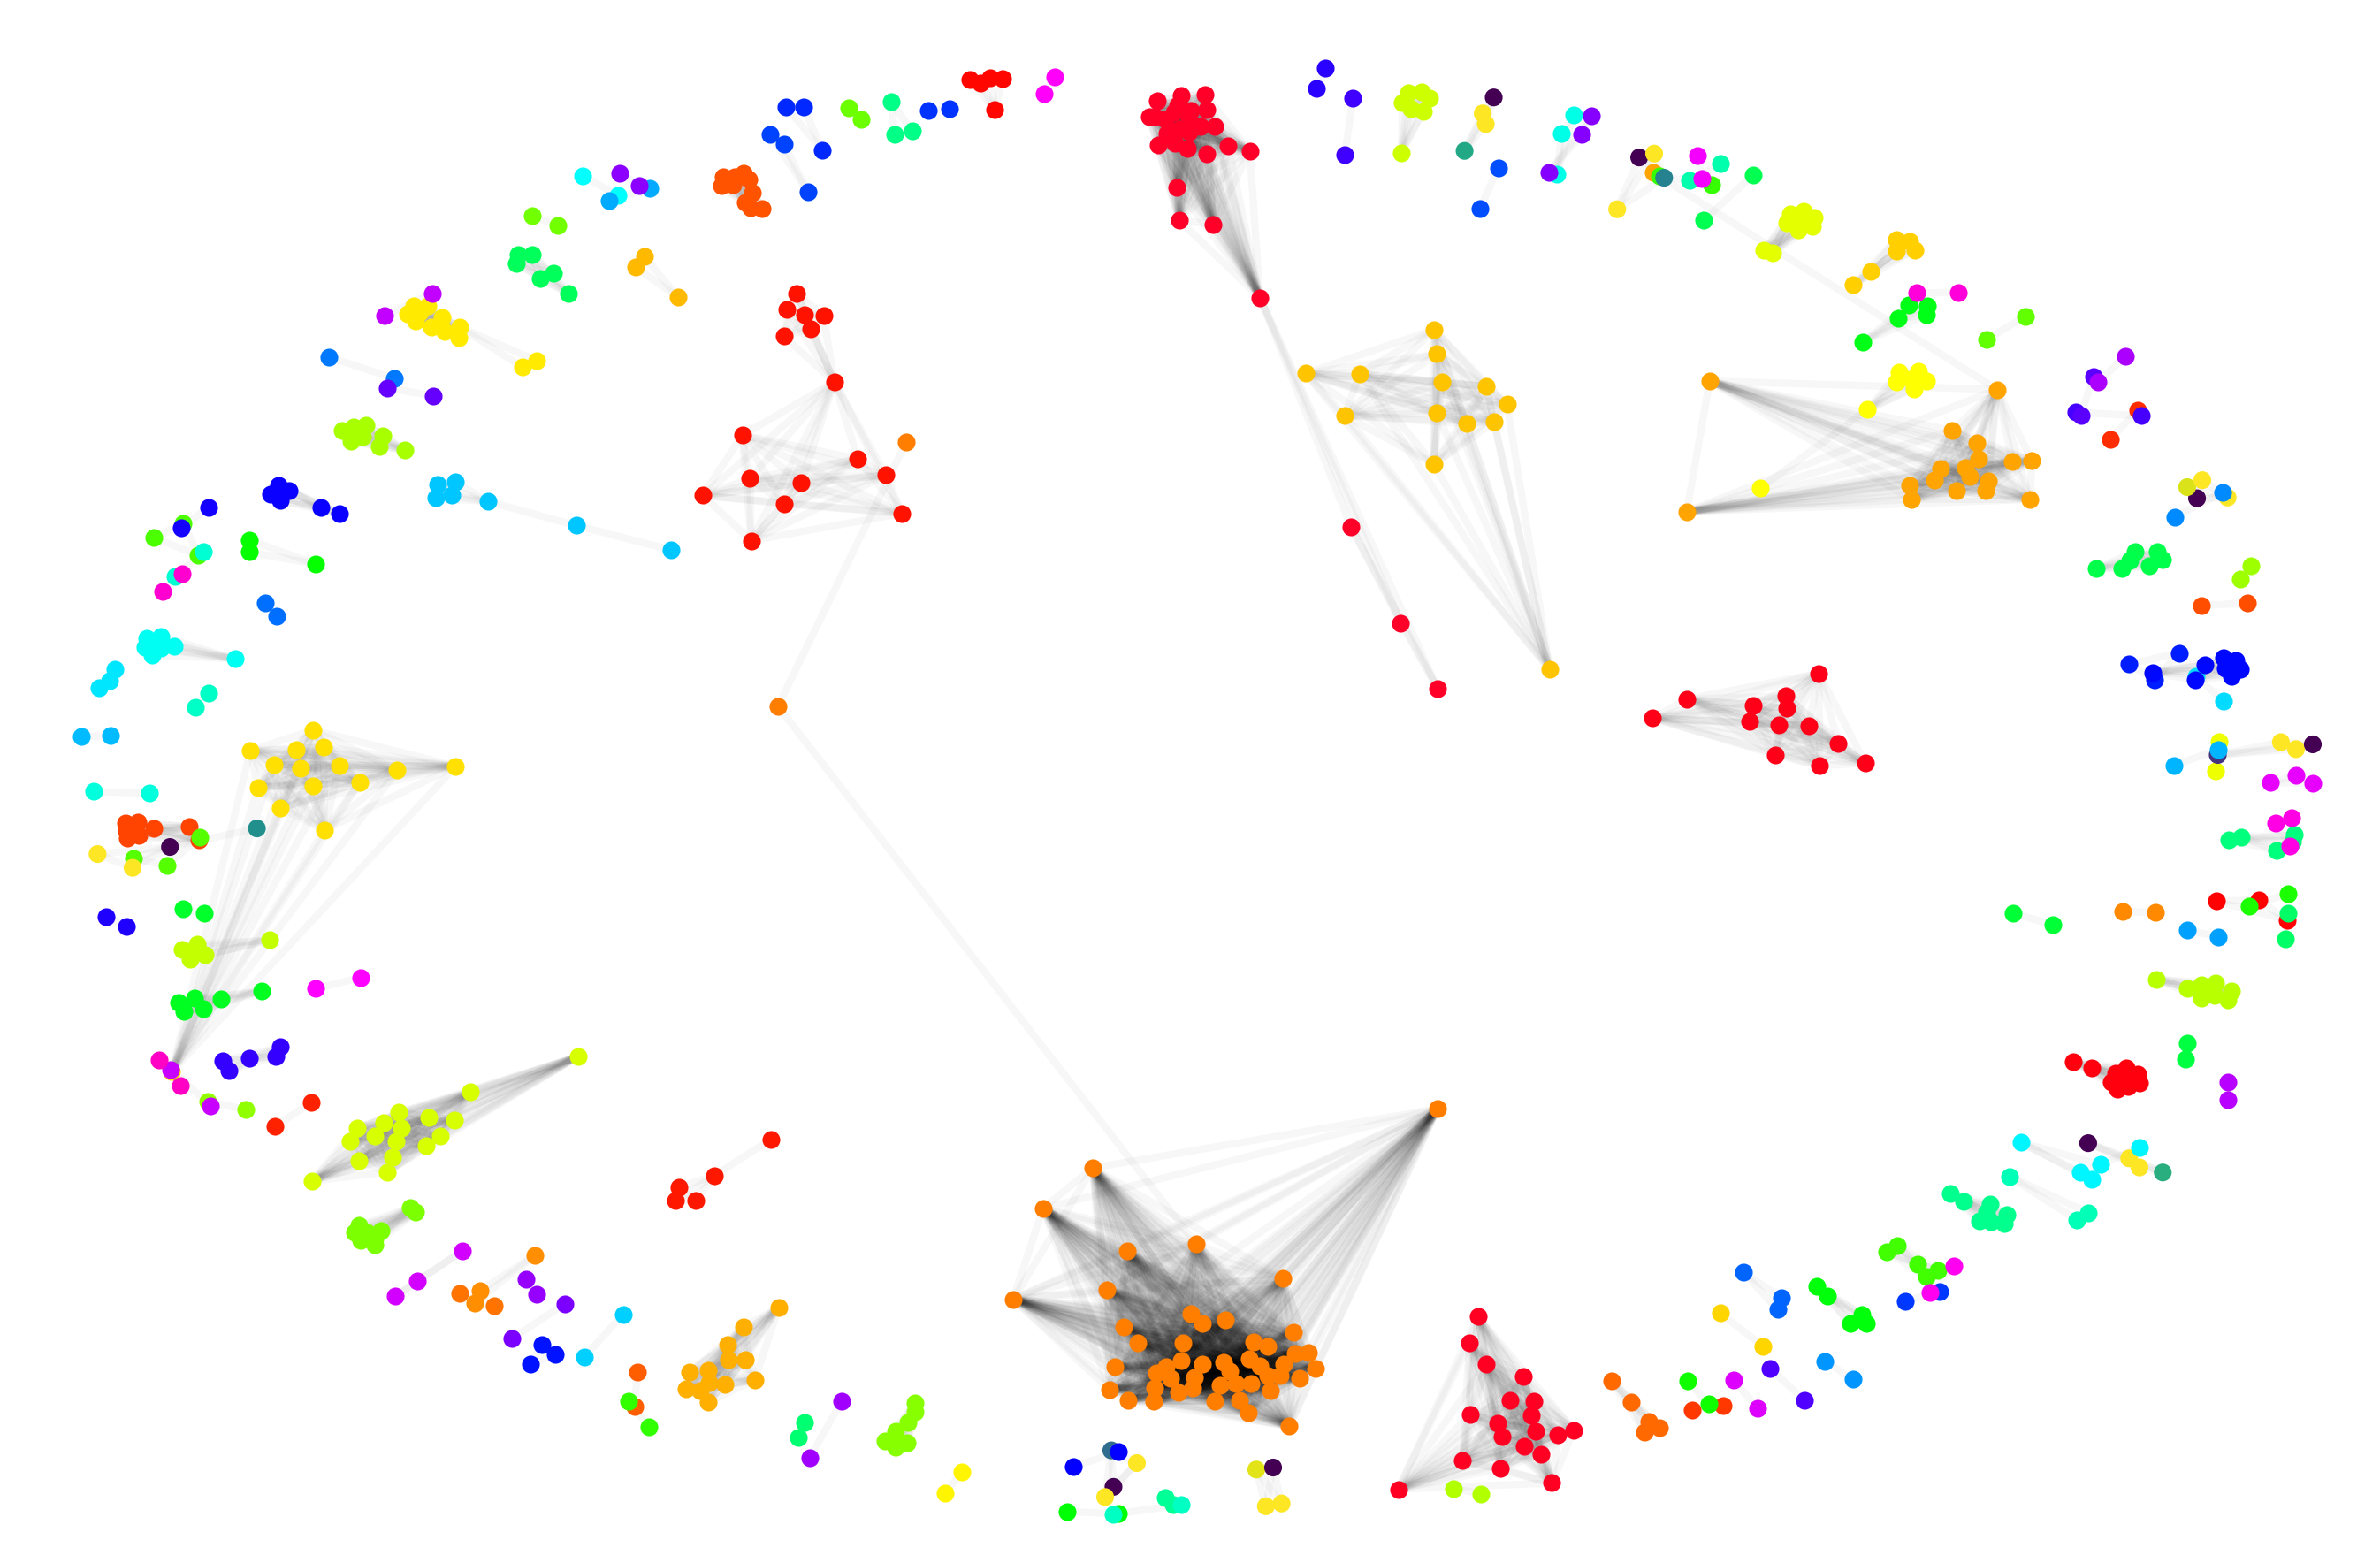
\includegraphics[width=.5\textwidth]{graphLoc.png}
			\caption{Graph of the terrorist attacks dataset}
			\label{fig:graph attacks}
		\end{center}
	\end{figure}
\end{frame}

\begin{frame}
\frametitle{Exploring The Data: Terrorist Attacks II}
	
	\begin{center}
	\includemedia[activate=pageopen,
  			      width=240pt,height=130pt,
  			      addresource=timelapseOfGraph.mov,
  			      flashvars={%
                               src=timelapseOfGraph.mov      % same path as in addresource! %&scaleMode=stretch % removes black bars
			      &autoPlay=true   % optional configuration
			      &loop=true          % variables
			      }]{\fbox{Click!}}{StrobeMediaPlayback.swf}
	\end{center}
	
	\begin{itemize}
		\item A lot of isolated nodes
		\item The sub-components are complete
	\end{itemize}
\end{frame}